\section{Encoding Attribute Sequences}
\label{sec:ordering}
In some applications, the \emph{order} of attributes is important.  For example, in service chaining, traffic must traverse middleboxes in specified order.  In this section, we extend our encoding scheme to support \textit{sequences} of attributes.  We first propose a simple representation of the attribute sequences in a sequence graph.  Next, we discuss how to encode sequences when the attributes follow a partial order.  Then, we show how to encode sequences in general, even when the attributes do not form a partial order.

\subsection{Graph of Attribute Sequences}
Based on the required sequences the sequence graph $G$ can be constructed with nodes representing attributes. A directed edge from a node $u$ to a node $v$ exists if $u$ appears in adjacency before $v$ in one of the sequences.  

\begin{table}
    \begin{tabular}{| l | l | l |}
    \hline
    Attribute & Unordered Match & Ordered Match\\ \hline
    A & $1011**$ & $1011**$ \\ \hline
    B & $101*1*$ & $10101*$ \\ \hline
    C & $101**1$ & $101001$ \\
    \hline
    \end{tabular}
    \caption{Wildcard strings for ordered versus unordered attributes. %In the unordered case, the string matches if the target attribute bit is 1, and does not depend upon the bits of other attributes.
     In the ordered case, the string only matches if the target attribute bit is 1 and all bits for attributes preceding the target attribute are 0. This ensures only matching on the next attribute in the ordering succeeds.} 
    \label{tab:ordering}
\end{table}

\subsection{Aligned Ordering Constraints}
We first assume that the attributes follow some (partial) order. In this case there exists a sequence of all attributes such that all input sequences can be derived as a subsequence of it. 
We refer to such a sequence as a supersequence. 
In such a case the sequence graph $G$ is a DAG (directed acyclic graph), i.e. it has no cycles.

A supersequence can be found by processing the DAG's nodes in order. Then, sequencess are selected, each as the union of some input sequences. A tag of a sequence would then include  identifier together with a mask of its attributes based on the order of the supersequence. 
Table \ref{tab:ordering} illustrates an example of  wildcard rules imposing such an ordering for a sequence with attributes $A, B, C$ that was assigned the identifier $101$. 
If the ordering dictates that an attribute $B$ must appear after $A$, then any wildcard rule for decoding $B$ must check that the $B$ bit is 1 and the $A$ bit is 0. This causes the wildcard rule to only successfully match if no other attributes that come before $B$ appear in the set. %In other words, testing for $X$ only returns true if tests for all attributes before $X$ returns false. 

\subsection{Not-Aligned Ordering Constraints}
Sometimes, there does not exist a supersequence of attributes that all sequences follow its order. This is case  if for two attributes $B, A$,  $B$ appears before $A$ in some sequences, but $A$ appears before $B$ in others. Similarly, this happens when $B$ appear before $A$ in a sequence and $A$ has to appear before $B$ based on transitivity of other attributes. We refer to that as order-inconsistency.  In such cases the graph $G$ contains a cycle. We describe two approaches to deal with this scenario. 

\textbf{Approach I:} The first approach begins with the input sequences. In each step, pairs of supersets are considered as long as their merging does not result in order-inconsistency. A pair is selected based on similar criterions as for the non-ordered sets. Finally, for each superset in the result, an identifier is allocated based on a potential order of the corresponding attributes.

\textbf{Approach II:} The first approach can sometime result in a large number of sequences that cannot be further merged. The second approach is more flexible by allowing the merging of two sequences even if this results in order-inconsistency. We solve the inconsistency by finding a supersequence with multiple appearances of some of the attributes such that merged sequences can be described as subsequences. 

To do so systematically, we construct the sequence graph $G$, shown in \ref{fig:ordering}(b) for the sequences  in \ref{fig:ordering}(a). We then run an algorithm for finding Strongly Connected Components (SCCs) on this graph. A strongly connected component is a set of nodes such that for every pair of nodes $u$ and $v$ in the set, $u$ has a path to $v$ and vice versa. In this context, every SCC corresponds to a set of incomparable elements.  Figure \ref{fig:ordering}(d) and (e) shows the result of using this new ordering to modify each sequence.  
Figure \ref{fig:conflict_res} details the process for determining which elements to split to create a new, totally ordered universe.


\begin{figure}[t!] 
\begin{minipage}{1\linewidth}
\begin{subfigure}[c]{0.96\linewidth}
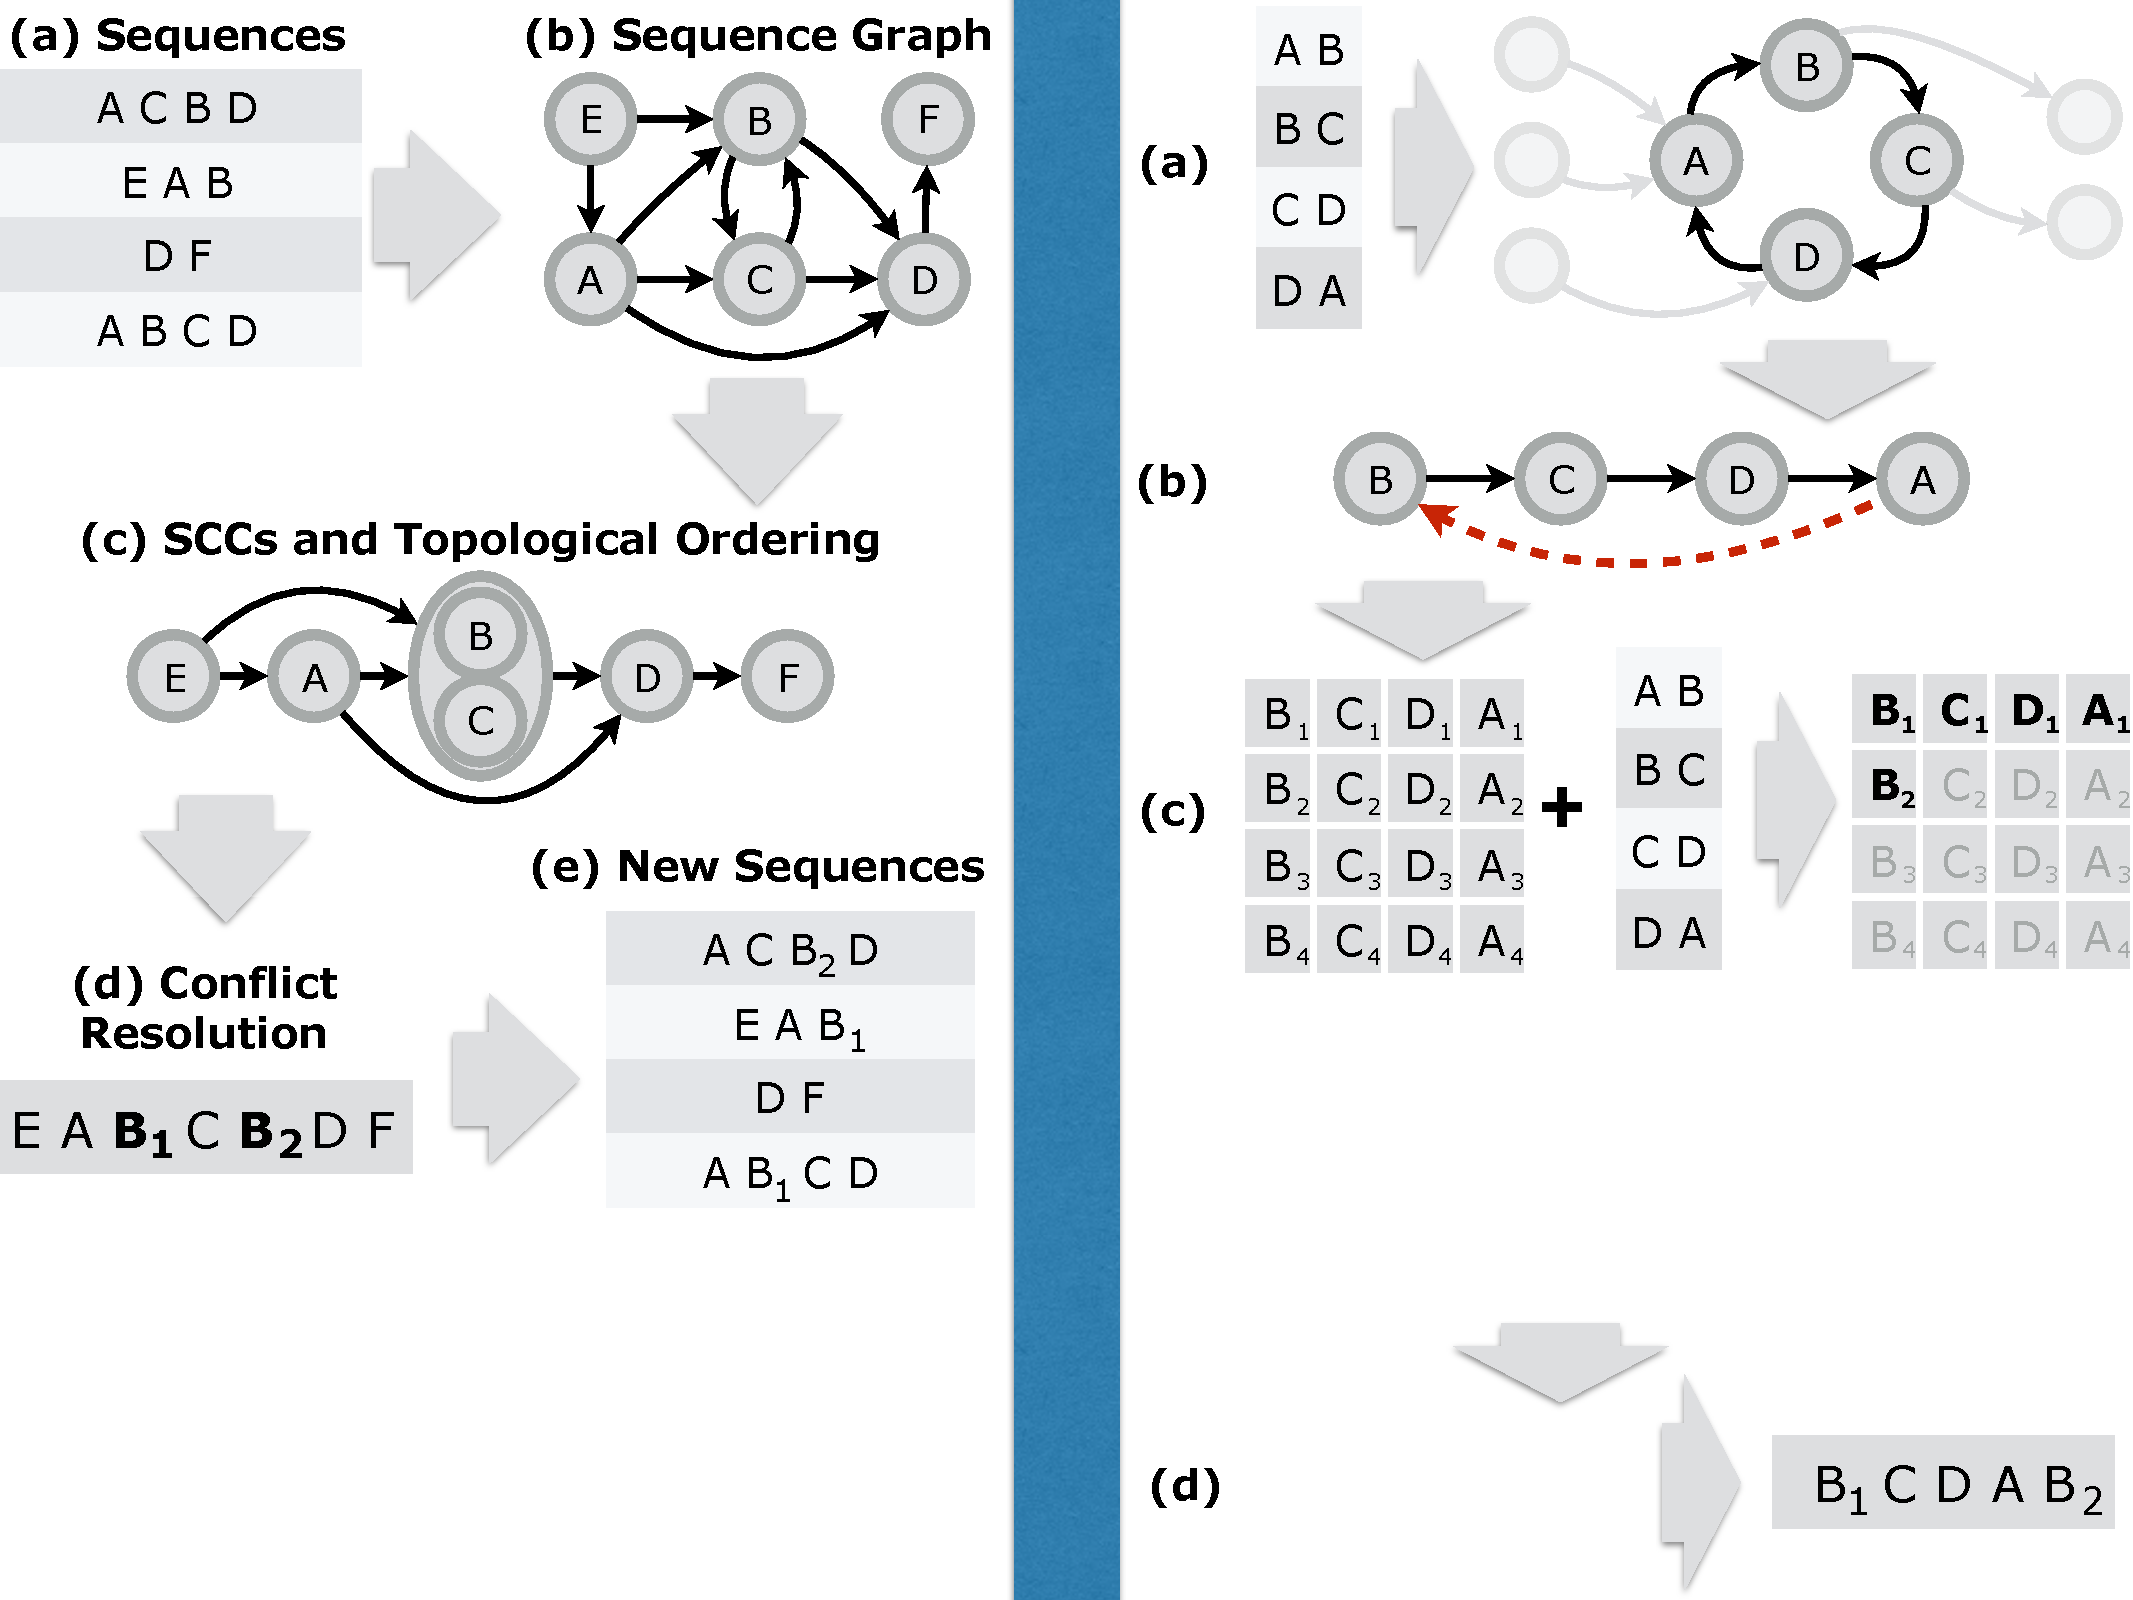
\includegraphics[trim={0 6cm 19.2cm 0}, clip, width=\linewidth]{figures/partial_ordering}
\end{subfigure} 
\end{minipage} 
\caption{Not-aligned ordering constraints. (a) shows the four input ordered sequences. In (b) illustrates the corresponding sequence graph $G$.. (b) shows the disjoints SCCs  (Strongly Connected Components) of $G$. Each SCC corresponds to a set of incomparable elements. (d) describes the result of splitting elements to resolve order-inconsistency, which is covered in more depth in figure \ref{fig:conflict_res}. In (e), the original sequences are modified with the splits such that each sequence adheres to the constructed ordering.}
\label{fig:ordering}
\end{figure}



\begin{figure}[t!] 
\begin{minipage}{1\linewidth}
\begin{subfigure}[c]{0.96\linewidth}
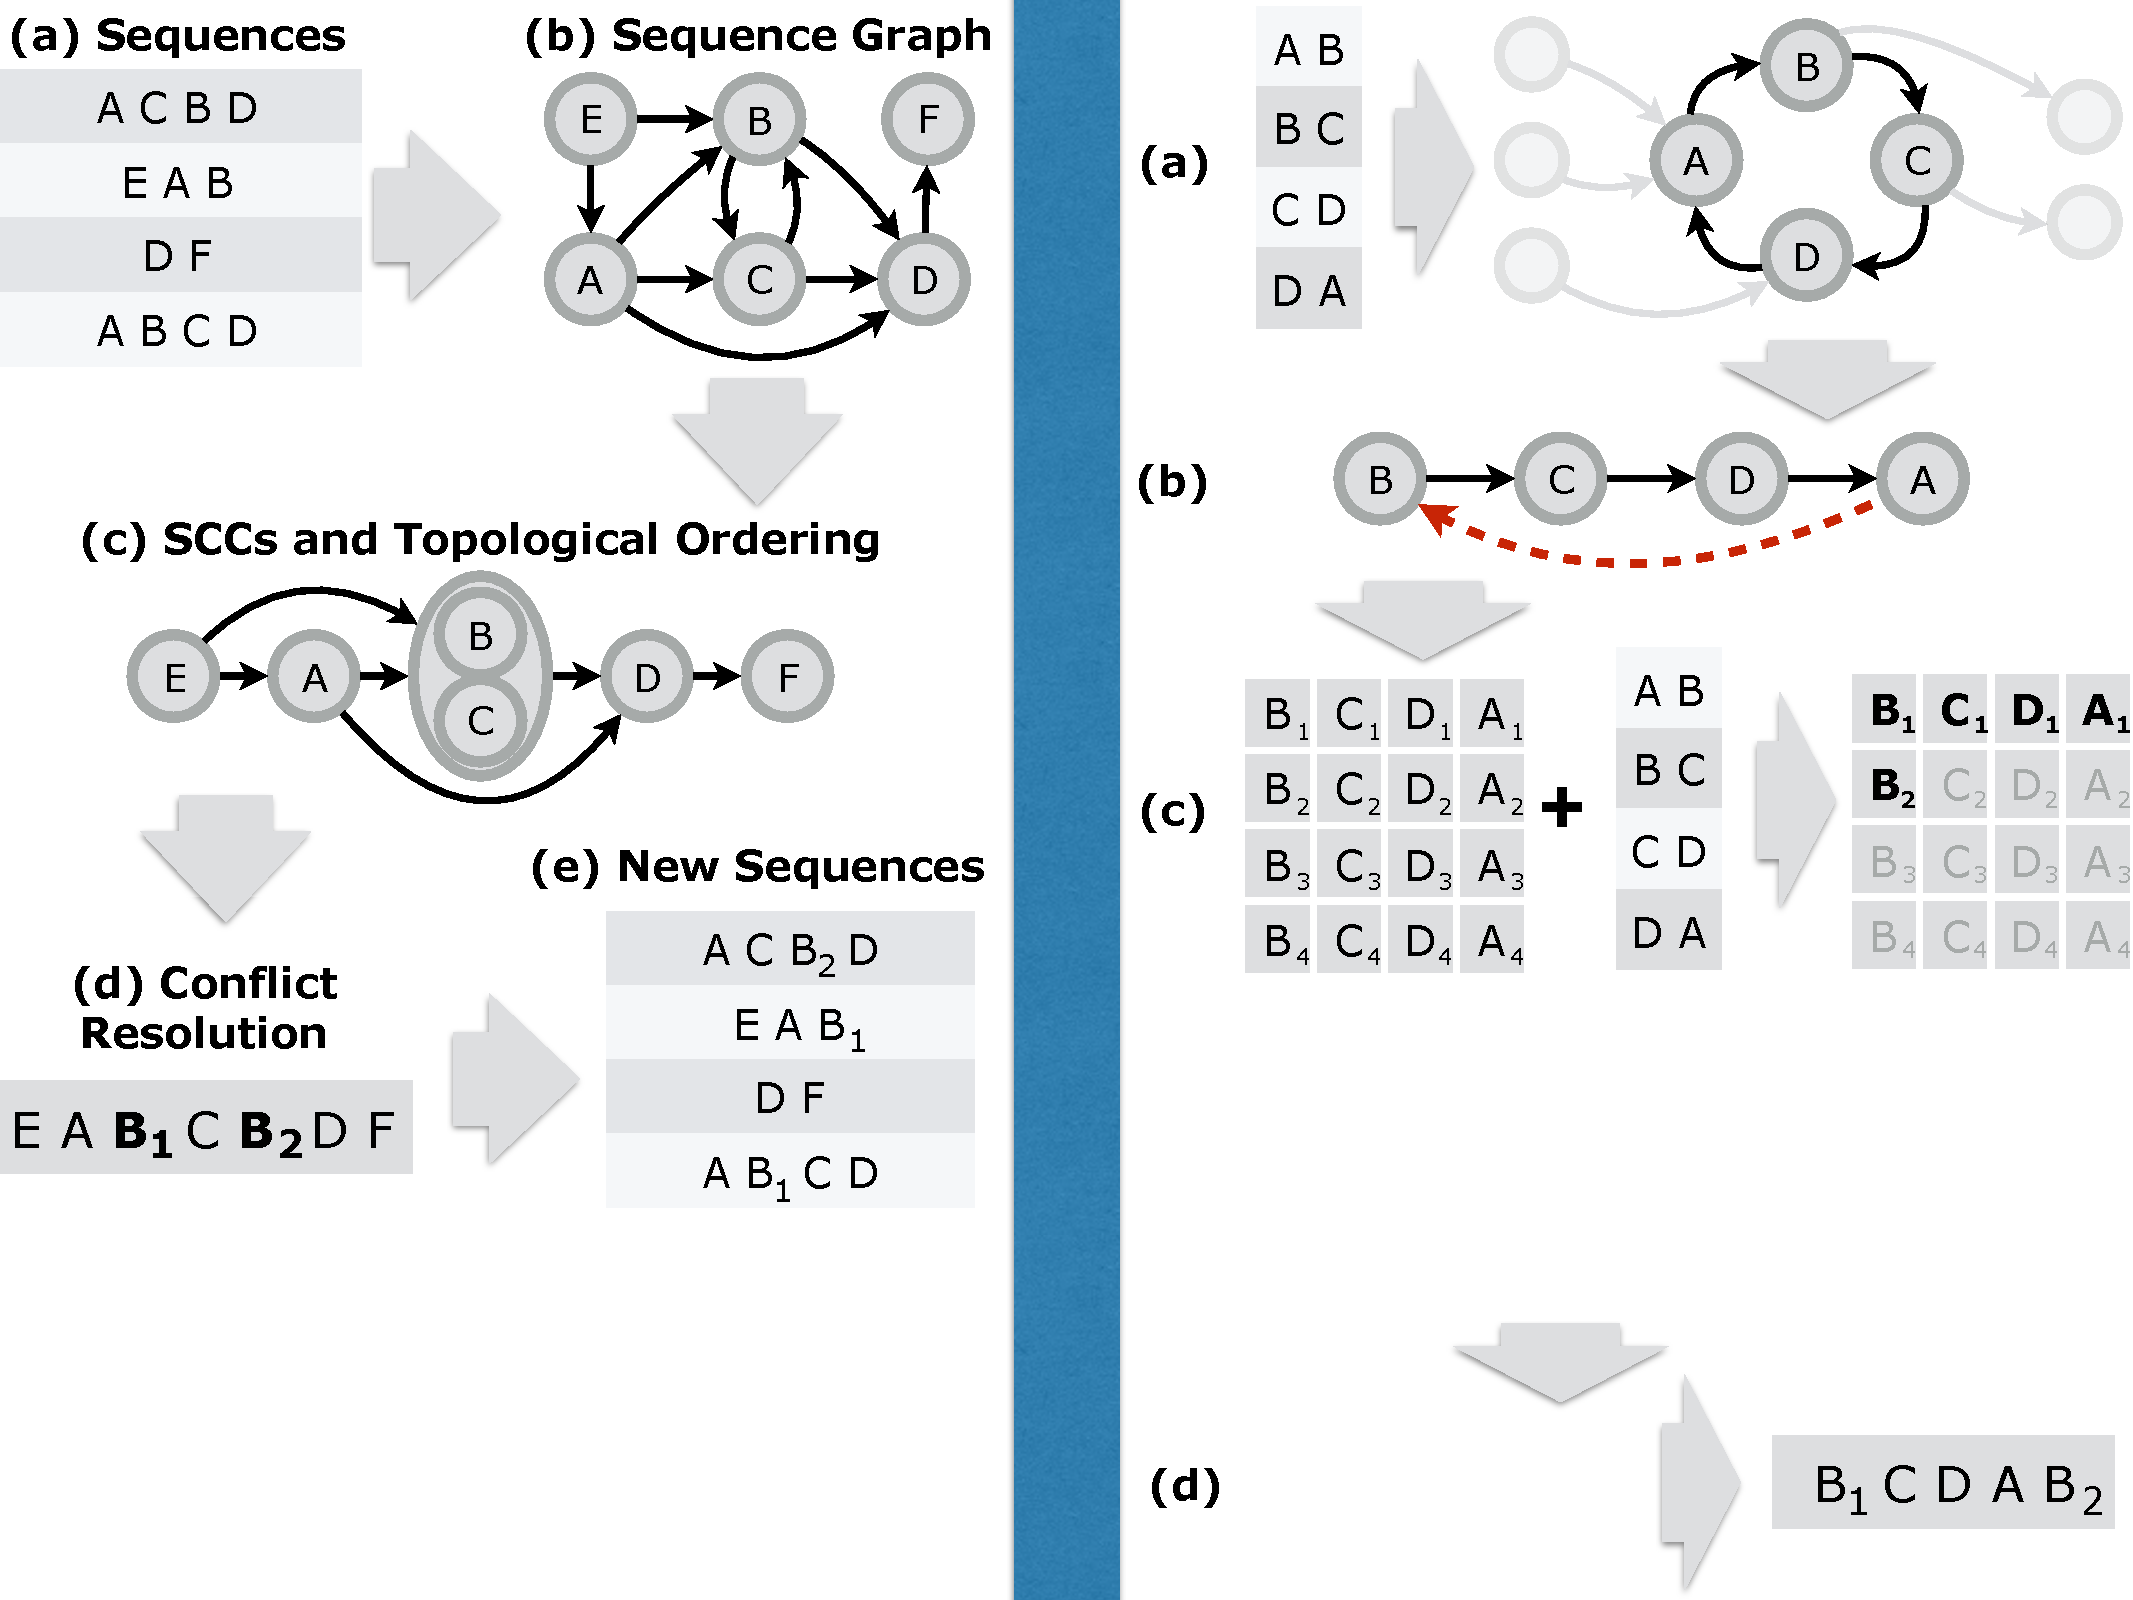
\includegraphics[trim={19.2cm 10cm 0 0}, clip, width=\linewidth]{figures/partial_ordering}
\end{subfigure} 
\end{minipage} 
\caption{This details the order-inconsistency resolution step of the algorithm. (a) shows a SCC of four attributes. (b) shows an 'almost' ordering of the SCC nodes, which minimizes the number of backward edges. (c) shows a  construction of a worst-case quadratically-sized universe, which is then traversed by every sequence to determine which attributes to splits for the new ordering.}
\label{fig:conflict_res}
\end{figure}
 

